% This file was converted to LaTeX by Writer2LaTeX ver. 1.2
% see http://writer2latex.sourceforge.net for more info
\documentclass[twocolumn,letterpaper]{article}
\usepackage[utf8]{inputenc}
\usepackage[T1]{fontenc}
\usepackage[english]{babel}
\usepackage{amsmath}
\usepackage{amssymb,amsfonts,textcomp}
\usepackage{color}
\usepackage{array}
\usepackage{hhline}
\usepackage{hyperref}
\hypersetup{dvips, colorlinks=true, linkcolor=blue, citecolor=blue, filecolor=blue, urlcolor=blue}
\usepackage[dvips]{graphicx}
% Outline numbering
\setcounter{secnumdepth}{0}
% List styles
\newcommand\liststyleLii{%
\renewcommand\theenumi{\arabic{enumi}}
\renewcommand\theenumii{\arabic{enumii}}
\renewcommand\theenumiii{\arabic{enumiii}}
\renewcommand\theenumiv{\arabic{enumiv}}
\renewcommand\labelenumi{\theenumi.}
\renewcommand\labelenumii{\theenumii.}
\renewcommand\labelenumiii{\theenumiii.}
\renewcommand\labelenumiv{\theenumiv.}
}
\newcommand\liststyleLi{%
\renewcommand\theenumi{\arabic{enumi}}
\renewcommand\theenumii{\arabic{enumii}}
\renewcommand\theenumiii{\arabic{enumiii}}
\renewcommand\theenumiv{\arabic{enumiv}}
\renewcommand\labelenumi{\theenumi.}
\renewcommand\labelenumii{\theenumii.}
\renewcommand\labelenumiii{\theenumiii.}
\renewcommand\labelenumiv{\theenumiv.}
}
% Page layout (geometry)
\setlength\voffset{-1in}
\setlength\hoffset{-1in}
\setlength\topmargin{0.7874in}
\setlength\oddsidemargin{0.7874in}
\setlength\textheight{9.4251995in}
\setlength\textwidth{6.9251995in}
\setlength\footskip{0.0cm}
\setlength\headheight{0cm}
\setlength\headsep{0cm}
% Footnote rule
\setlength{\skip\footins}{0.0469in}
\renewcommand\footnoterule{\vspace*{-0.0071in}\setlength\leftskip{0pt}\setlength\rightskip{0pt plus 1fil}\noindent\textcolor{black}{\rule{0.25\columnwidth}{0.0071in}}\vspace*{0.0398in}}
% Pages styles
\makeatletter
\newcommand\ps@Standard{
  \renewcommand\@oddhead{}
  \renewcommand\@evenhead{}
  \renewcommand\@oddfoot{}
  \renewcommand\@evenfoot{}
  \renewcommand\thepage{\arabic{page}}
}
\newcommand\ps@FirstPage{
  \renewcommand\@oddhead{}
  \renewcommand\@evenhead{}
  \renewcommand\@oddfoot{}
  \renewcommand\@evenfoot{}
  \renewcommand\thepage{\arabic{page}}
}
\makeatother
\pagestyle{Standard}
\title{}
\author{}
\date{2012-10-21}
\begin{document}
\clearpage\setcounter{page}{1}\pagestyle{Standard}
\thispagestyle{FirstPage}
{\centering
Information Security:
\par}

{\centering
A cornerstone in teaching online usage
\par}

\clearpage
\bigskip

{\centering
Victor Rudolfsson
\par}

{\centering
Høgskolen i Gjøvik
\par}


\bigskip

The amount of people connected to the internet grows continuously, and as more and more people get connected, more
threats appear to a greater number of people. However, whereas corporations and organizations in many cases have
realized the need to educate their employees in information security to a certain extent to ensure the security of
their data, end users have not reached the same level of understanding of how oneself is the key to a secure system.
For many end-users, installing an anti-virus software seems sufficient to be secure – although anti-virus software may
help the user to stay safe from certain kinds of malware, it is in the end up to the user to avoid them in the first
place. Should safe online usage and education perhaps be taught in a far earlier stage than at the corporate level to
create safe internet usage habits before unsafe ones are already in place?

\subsection[Teaching computer literacy at a young age]{\bfseries \textup{Teaching computer literacy at a young age}}
About ten to fifteen years ago it wasn't uncommon to have basic IT classes in primary school, if only to introduce the
young students to the new phenomena called 'the internet', at the age of 7-10. These basic classes served to teach a
young student how to access information online, and how to use search engines to find information, since this would be
crucial knowledge later on in their lives. As the internet became a more common commodity in most peoples households,
and students were more or less expected to be exposed to it at home, these classes either faded, stayed the same or
scaled poorly in regards to security.

These classes could still prove useful today, and whereas some countries invest heavily in increasing their populations
computer literacy from a young age \textsuperscript{[1]}, security rarely seems to be one of the core values of such
education. IT education in primary schools should aim to incorporate basic information security as a core value to a
certain degree, to teach the user how to recognize potential threats and avoid them, and to realize that the biggest
security threat in an information system is more often than not the user – even when the software and technology is
there as a complementary tool.

\subsection[Information loss: who is to blame?]{\bfseries \textup{Information loss: who is to blame?}}
With the internet of today, malware is not the only threat users are subject to online. Web sites that collect, store
and sell personal information can in many cases seem harmless – because they are trusted by the user
\textsuperscript{[2]}.\textbf{ }However, this is the same principle most malicious sites build on as well; gaining the
trust of the user.

It is important to know the risks of storing personal information with a website, as the user may not know how this
information is treated. What happens if this website encounters a security breach, for example – how much do you have
at stake? 

As a child, one of the most fundamental rules I was taught about online usage was to \textit{never give out personal
information such as name, address or similar}. This is something most online users consider part of their online
behavior today, and is becoming increasingly more common – and the usage of this information to build profiles about
users and sell this information has actually become a booming field over the past years\textsuperscript{[3]}.

Many malicious sites build on the same principle as safe sites; simply asking the user for information whilst giving the
user an impression of safety. What makes a site or application safe, is how they store, protect and treat your data –
which users should be able to find out in the website's \textit{Privacy Policy }\textsuperscript{[4]}.

To break it down even more, information can be lost in two ways: either it's stolen from the user, or the user
carelessly gives it away. It's up to the user to identify a risky situation. 

Because it is such a common practice by websites to request personal information these days, and for users to be
required to supply personal information in order to use a service, many users do not even contemplate what actually
happens to their information, or how it's dealt with. This opens up for malicious sites to more easily gain the trust
of users, as requesting personal information is no longer seen as questionable behavior. 

Even sites that are perceived as harmless – such as Facebook, Google, or Apple – could at one point prove to be the
exact opposite, in the event they suffer a security breach and your information is compromised. In the end, it's all
about trust – but if this trust is breached, it's important to know what you have at stake, and this is something users
should keep in mind before such a breach of trust occurs. 

\subsection[Privacy Policies]{\bfseries \textup{Privacy Policies}}
One of the cornerstones of teaching safe online usage is to teach the user how to become aware of how the information he
or she may supply is treated and retained, and why. Another important point is to teach the user how to identify
potentially untrustworthy websites. For websites that allow use by children below the age of 13, the \textit{Children's
Online Privacy Protection Act (COPPA) }requires sites to, amongst other things, publish a privacy statement that
presents information about how data is collected and used, such as what personal information is collected, whether or
not it will be shared by third parties, and how to contact someone at the web site who can answer any questions
regarding their privacy policy \textsuperscript{[4]}.

It is an integral part of safe online usage to be aware of how your information is used, and therefore the ways of which
one can become informed of it – and the importance of reading the privacy policy - should serve as a fundamental part
of education for children as they start using the internet. 

\subsection[Identifying links]{\bfseries \textup{Identifying links}}
One of the most common ways users come in contact with malware or malicious sites today is by clicking links they should
not have clicked. The risk is not always obvious, however – and the key to understanding the risk is to first
understand how to identify a sketchy link. 

A big part of questionable links come from advertisement, tempting the user to follow the link to a more malicious
website. The first step to identifying the threat posed by this link is to understand that the link comes from an
advertisement, and that just because the user considers the site viewed safe, does not mean the advertisement on the
site is necessarily safe. Studies have shown that when a websites credibility is supposedly high, users argue less with
the advertisements claim and the message has a greater impact\textsuperscript{[1]}. It is important to understand that
many sites use advertising services that generate advertisement independently of the site they're placed
on.\textsuperscript{[3]}

In recent years, the people behind such malicious links have become more and more crafty in making these links seem like
part of the original website and thereby gain false trust from the user (\textit{see attachment a for an example of an
ad blending in as a core element of a site}).

Knowing where advertisement is placed on a website, and how to know if a banner or hyperlink is advertisement or part of
the source website plays a key role in knowing what links to trust, and simple ways of deciding this should be taught
as part of basic computer literacy classes – for example by hovering the cursor over the banner or hyperlink, and
comparing the URL shown in the status bar of the browser with the one shown in the address bar; teaching the user to
react accordingly if the URLs are fundamentally different, or the URL shown in the status bar contains words related to
advertisement business. 

\subsection[Effective password creation habits]{\bfseries \textup{Effective password creation habits}}
A key part, literally, in keeping ones information safe is usually by safeguarding it with a password. It's no new idea
that users should use a different password on every site - but passwords are used in such a big portion of services
online, that it becomes virtually impossible for users to use a different password for every single service they use.
Therefore a sustainable, scalable password policy should be taught so that it forms a habit – preferably even before
using passwords become a habit – to create passwords that are inherently different for every site, but using a pattern
that makes it easy to remember. For example, writing your favorite food, or your favorite quote, with every vowel
replaced with a number resembling that vowel, ending with the name of the website it's used on, and separating every
word with a special character (for example, if my favorite quote was “A poet can survive everything but a misprint”, a
password for my Google account could be “\textit{4\&p03t\&c4n\&surv1v3\&4nyth1ng\&but\&4\&m1spr1nt\&g00gl3}”).

By using such patterns, and making it a habit even before using passwords has become a habit, guessing a password could
become significantly more complicated for a potential attacker. However, one should also remember that the amount of
characters in a users password could play a similar role in strengthening it, and simply using a lot of characters
could just as well make a users password stronger – whether or not it contains special characters. 

Teaching the importance of privacy and safety online at a young age could help to reduce the amount of malware infected
systems, and raise the general awareness about the risks one takes when browsing the internet. This could greatly
reduce the workload in several areas such as law enforcement by reducing the amount of requests they have to deal with,
IT helpdesks and IT recovery, and so on – but more importantly, it would reduce the amount of loss suffered by the
average user in a preventive manner rather than a post-incident manner.

Internet usage taught at a young age should teach online usage from a safety perspective, where sound habits are formed
with privacy and security in mind \textsuperscript{[7]}. IT education for young students should aim to create effective
habits in keeping private data confidential by teaching sound password creation and memorization habits, teaching the
student how to learn about a sites privacy policy and the importance of it, and how to distinguish between threats, and
non-threats – as well as identifying that threats are out there. 

Not only should the user learn to approach content with thinking before clicking – but also questioning before
submitting. Why exactly does a given website require certain information from the user, and what will happen to it? 

\subsection[References]{\textmd{\textup{References}}}

\bigskip


\bigskip

\liststyleLii
\begin{enumerate}
\item Tiger Leap Foundation, Estonia, \url{http://www.tiigrihype.ee/et/uudised/programmeerimine-jouab-iga-koolilapseni}
\item “\textit{Location, Location, Location: Insights for Advertising Placement on the Web}”, July 01 2001, Journal of
Advertising Research, Shamdanasi, Prem N.; Stanaland, Andrea J. S; Tan, Juliana
\item Arshad Mohammed and Sara Kehaulani Goo, June 15, 2006
\url{http://msl1.mit.edu/furdlog/docs/washpost/2006-05-15_washpost_data_mining.pdf}
\item “\textit{A Privacy Policy Model for Enterprises}”, Gunter Karjoth and Matthias Schunter, IBM Research,
\url{http://semper.schunter.org/sirene/publ/KaSc02.privacyASL.CSFW02-final.pdf} 
\item Children's Online Privacy Protection Act of 1998 (\url{http://www.ftc.gov/ogc/coppa1.htm}) 
\item \textit{User-Generated Advertising, }United States Patent Application Publication US2009/0112685 A1,
\url{http://www.google.no/patents?vid=USPATAPP11925250&printsec=abstract}
\item “\textit{Facebook and Online Privacy: Attitudes, Behaviors, and Unintended Consequences}”, 17 Nov 2009, Volume 15,
pages 83–108 (http://onlinelibrary.wiley.com/doi/10.1111/j.1083-6101.2009.01494.x/pdf)
\end{enumerate}
\liststyleLi
\begin{enumerate}
\item[] 
\bigskip
\end{enumerate}

\bigskip

\clearpage
a. The blue download button is the correct one, whereas the green is advertisement designed to make a user click it
without knowing its content
\begin{figure*}
\centering
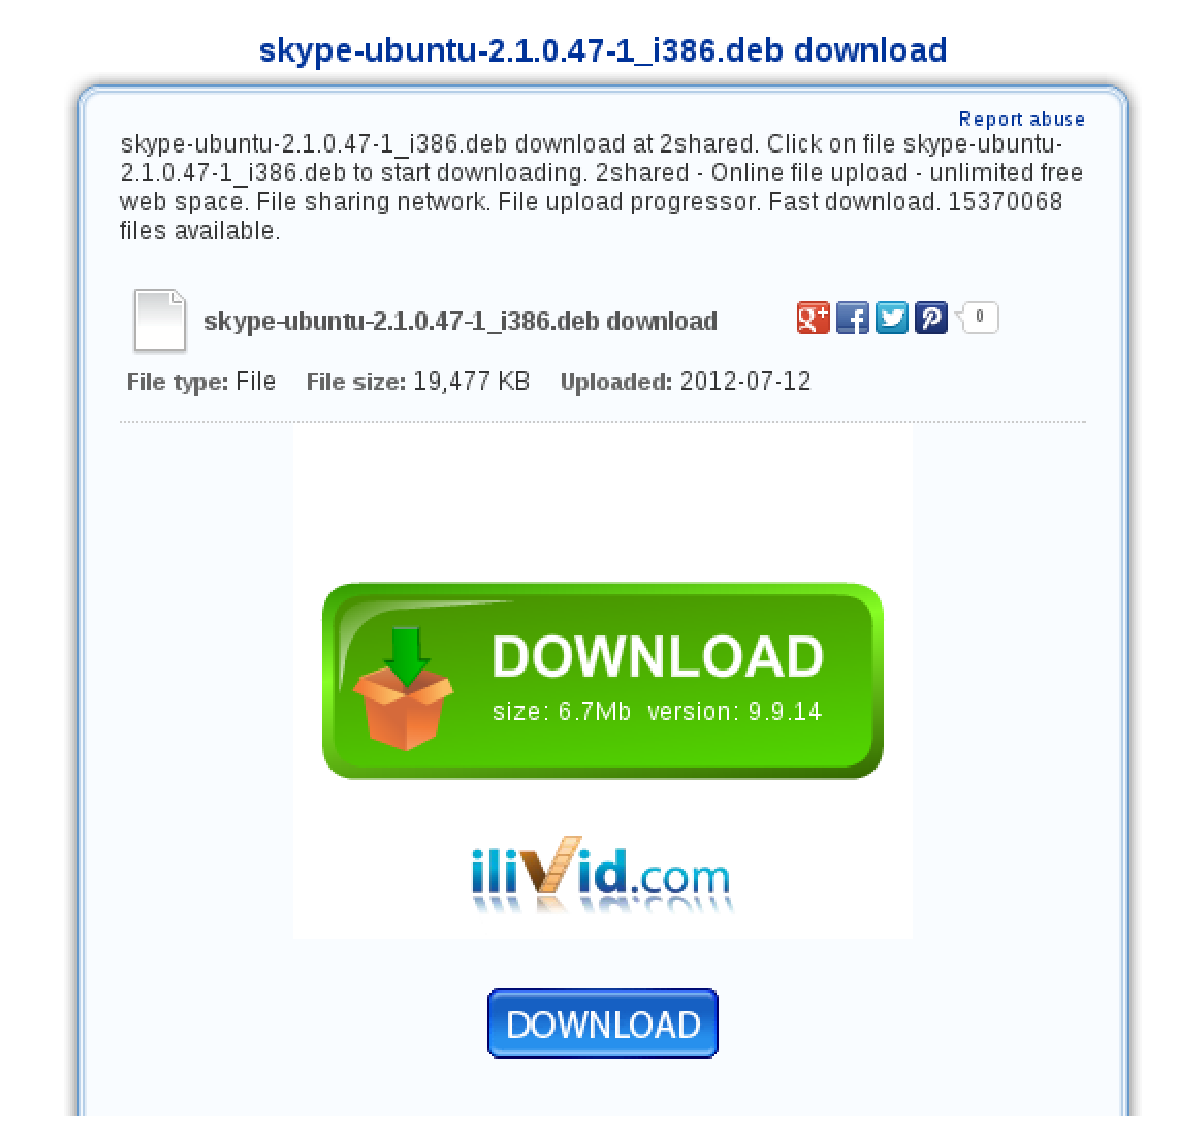
\includegraphics[width=5.8335in,height=5.552in]{education-img/education-img001.eps}
\end{figure*}
\end{document}
